% Main manuscript for Engineering with Computers (Springer svjour3)
\documentclass[smallextended]{svjour3}      % onecolumn (second format)
\smartqed  % flush right qed marks, e.g. at end of proof

% Packages
\usepackage{graphicx}
\usepackage{amsmath,amssymb}
\usepackage[numbers,sort&compress]{natbib}
\usepackage[hidelinks]{hyperref} % reviewer-friendly (no colored boxes)
\usepackage{microtype}
\usepackage{url}
\usepackage[switch]{lineno} % optional line numbers for review (toggle below)

% Review toggles
\newif\ifanonymous % set to \anonymoustrue for anonymous review copy
\anonymousfalse
\newif\ifwithlinenumbers % set to \withlinenumberstrue to enable line numbers
\withlinenumbersfalse

% Journal name
\journalname{Engineering with Computers}

% Metadata (edit as appropriate)
\title{A Condition--Driven Geometric Framework for Mesh Generation: Historical Mapping and Design Insights}

\titlerunning{A Condition--Driven Framework for Mesh Generation}        % if too long for running head

\ifanonymous
  \author{Anonymous}
  \authorrunning{Anonymous}
  \institute{Anonymous Institution}
\else
  \author{First Author \and Second Author}
  \authorrunning{First Author et al.}
  \institute{First Author \at\\Department, University, City, Country\\\email{first.author@example.com}
             \and
             Second Author \at\\Institute, University, City, Country}
\fi

\date{}

\begin{document}
\maketitle
\ifwithlinenumbers\linenumbers\fi

\begin{abstract}
Mesh generation underlies simulation, optimization, and engineering design, yet decades of algorithms are often compared in an ad-hoc manner. We propose a concise condition--driven geometric framework that decomposes a method into six modules: Input, Global Rule, Problem Reduction, Local Rule, Engine, and Output. Using this lens, we remap representative structured, unstructured, optimization-based, and field-guided methods from the 1960s to recent years, revealing cross-cutting patterns that explain success and failure modes. We further show how the framework can guide small but effective design patches, illustrated on advancing-front meshing. The framework clarifies what is reusable infrastructure and what is algorithm-specific policy, offering a path toward modular combinations and, ultimately, geometric agents for broader classes of problems.
\keywords{Mesh generation \and Delaunay triangulation \and quadrangulation \and hexahedral meshing \and CVT \and DistMesh \and advancing front \and mixed-integer quadrangulation \and field-aligned meshing \and problem reduction}
\end{abstract}

% Sections
% 1. Introduction
\section{Introduction}
Mesh generation is a critical enabler for computational physics, simulation-based design, and engineering software. Despite a long history and a diversity of algorithmic families, practitioners still lack a unified way to structure, compare, and recombine methods. As a result, engineers frequently rely on experience to select or tweak codes, making systematic improvement difficult.

This paper proposes and applies a simple but expressive six-part condition--driven geometric framework. We show that classical and modern meshing methods can be consistently aligned with this decomposition, and that the alignment exposes structural strengths, weaknesses, and recurring patterns across families. We further demonstrate that the framework is not merely retrospective: it can guide light-weight design patches that improve robustness without heavy re-engineering.

Our contributions are threefold:
\begin{itemize}
  \item We present a unified six-part framework for meshing: Input, Global Rule, Problem Reduction, Local Rule, Engine, and Output.
  \item We systematically remap major families---structured/PDE-based, advancing front, Delaunay and refinement, quadtree/octree, quadrangulation and hexahedral meshing, optimization- and field-guided methods---to this framework, highlighting module-level contrasts.
  \item We extract cross-cutting patterns (e.g., strength of problem reduction, global vs local dominance, hard constraints vs soft preferences, engine completeness) and illustrate a framework-guided patch for advancing-front meshing.
\end{itemize}

% 2. Scope and Problem Setting
\section{Scope and Problem Setting}
We focus on mesh generation as a condition--driven geometric construction problem: given a geometric domain, boundary constraints, and quality/size goals, construct a mesh that satisfies hard constraints while best achieving soft preferences. We do not address PDE solution on meshes nor general geometric recognition; our scope is the construction of 2D/3D meshes (triangular/quadrilateral and tetrahedral/hexahedral) under practical engineering requirements.

We view the problem family as:
\begin{quote}
Boundary description + quality targets + size control $\Rightarrow$ mesh.
\end{quote}
Hard constraints (Global Rule) include validity (no overlaps, proper adjacency), full coverage, and boundary conformity. Soft preferences include smooth element size transitions, shape quality, alignment to directions, and regularity of valence. The goal of this paper is not to invent a universal algorithm but to provide a structured perspective that clarifies what to reuse, what to optimize, and where algorithms tend to fail.

% 3. A Condition--Driven Geometric Framework
\section{A Condition--Driven Geometric Framework}
We decompose any meshing method into six modules that translate \emph{conditions} into a \emph{geometric solution}:
\begin{enumerate}
  \item \textbf{Input} (data, problem definition): domain geometry and task specification.
  \item \textbf{Global Rule}: hard constraints that no method may violate (topological validity, non-overlap, boundary conformity, etc.).
  \item \textbf{Problem Reduction}: mapping the task to a simpler or already-solved problem (e.g., ``triangulate first, then convert to quads''). This step also detects conflicts between the problem definition and the global rules (infeasibility).
  \item \textbf{Local Rule}: algorithm-specific heuristics or policies (e.g., edge flips, front selection, templates).
  \item \textbf{Engine}: the driver that repeatedly applies rules to reach an \emph{objective} using a specific \emph{method} (incremental construction, global optimization, or physical relaxation).
  \item \textbf{Output}: the resulting mesh.
\end{enumerate}

Figure~\ref{fig:framework} summarizes the information flow.

\begin{figure}[t]
  \centering
  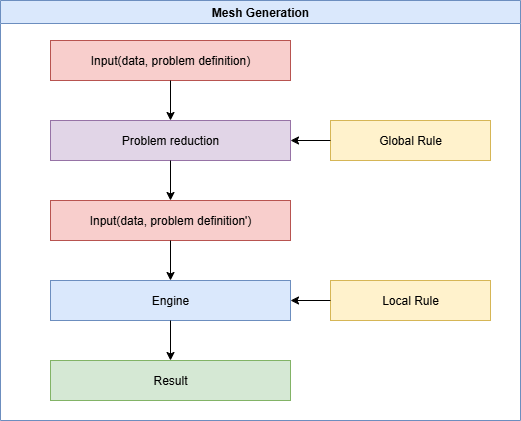
\includegraphics[width=0.9\linewidth]{figures/fw.png}
  \caption{The condition--driven framework: Input $\to$ Global Rule $\to$ Problem Reduction $\to$ (reduced Input) $\to$ Local Rule $\to$ Engine $\to$ Output.}
  \label{fig:framework}
\end{figure}

This lens foregrounds: (i) local vs global responsibilities; (ii) hard constraints vs soft preferences; and (iii) which modules are reusable infrastructure versus algorithm-specific policy. In the following sections we use this decomposition to remap historical families and extract design insights.

% 4. Historical Mapping of Mesh Generation Methods
\section{Historical Mapping of Mesh Generation Methods}
We briefly remap representative methods to the six-part framework; details and pointers appear inline.

\subsection{Structured mapping and PDE-based grids (1960s--1970s)}
\textbf{Conformity:} largely global; local rules are implicit in PDE discretization.
\\\textbf{Input:} boundary geometry, target spacing; often a mapping between physical and computational domains.
\\\textbf{Global Rule:} structured topology, boundary alignment, no overlaps.
\\\textbf{Problem Reduction:} transform meshing into solving elliptic PDEs or smooth mappings \citep{thompson1985grid}.
\\\textbf{Local Rule:} none explicit; positions result from global solves.
\\\textbf{Engine:} numerical solution (e.g., Laplace) until smooth coordinates emerge.
\\\textbf{Output:} structured quad/hex meshes; high quality but limited flexibility for complex topology.

\subsection{1980s: Advancing front, Delaunay, quadtree/octree}
\paragraph{Advancing front.} Incrementally fills the domain from the boundary. Strong Local Rule, weak explicit reduction. Robust near boundaries, can struggle with dead cavities.
\\\textbf{Input:} discretized boundary, size field.\
\textbf{Global Rule:} fill without overlaps, maintain the moving front.\
\textbf{Problem Reduction:} none explicit.\
\textbf{Local Rule:} heuristic front selection and point placement.\
\textbf{Engine:} iterative addition of elements.

\paragraph{Delaunay triangulation (Bowyer--Watson).} Direct solve with clear local criterion; reduction is implicit through computational geometry \citep{bowyer1981computing,watson1981computing}.
\\\textbf{Input:} point set (+ boundary constraints for CDT).\
\textbf{Global Rule:} coverage, CDT constraints.\
\textbf{Problem Reduction:} none explicit.\
\textbf{Local Rule:} empty circumcircle; local edge flips maintain Delaunay.\
\textbf{Engine:} incremental insertion.

\paragraph{Quadtree/octree subdivision.} Recursive space partitioning acts as explicit reduction \citep{yerry1983modified}.
\\\textbf{Input:} boundary and size thresholds.\
\textbf{Global Rule:} coverage and balance between neighboring levels.\
\textbf{Problem Reduction:} recursive subdivision to simple blocks.\
\textbf{Local Rule:} split/balance predicates.\
\textbf{Engine:} refine to leaves then convert to elements.

\subsection{1990s: Quality refinement, all-quad, and all-hex}
\paragraph{Delaunay refinement (Chew, Ruppert).} Elevates minimum-angle constraints to hard rules; reduction via iterative elimination of bad elements \citep{ruppert1995delaunay}.
\\\textbf{Input:} PSLG, angle threshold.\
\textbf{Global Rule:} boundary conformity and minimum-angle guarantee.\
\textbf{Problem Reduction:} repeated local repairs to remove skinny triangles.\
\textbf{Local Rule:} circumsenter insertion; protected splitting when invading constraints.\
\textbf{Engine:} refine until no bad elements remain.

\paragraph{All-quad meshing (Paving, Q-Morph).} Either direct layered fronts (Paving) or indirect conversion from triangles (Q-Morph). Q-Morph makes reduction explicit by first triangulating, then locally merging pairs of triangles into quads \citep{owen1998qmorph}.

\paragraph{All-hex (Plastering).} 3D layered fronts; partial conformity to the framework with possible engine failure in complex regions.

\subsection{2000s: Optimization and relaxation}
\paragraph{Centroidal Voronoi tessellations (CVT/Lloyd).} Optimize point locations then triangulate, emphasizing soft preferences via an energy objective \citep{du1999centroidal,lloyd1982least}.
\\\textbf{Engine:} alternate global Voronoi update with local centroid relocation.

\paragraph{DistMesh.} Spring system relaxation with Delaunay reconnections \citep{persson2004simple}. Reduction is implicit via energy minimization.

\subsection{Field-guided and parameterization-based (2010s)}
\paragraph{Mixed-Integer Quadrangulation (MIQ).} Convert layout to cross-field and parameterization optimization, then extract quads \citep{bommes2009mixed}.

\paragraph{Instant Field-Aligned Meshes.} Fast, greedy field-aligned layout: approximate reduction plus strong local decisions \citep{jakob2015instant}.

% 5. Cross-cutting Patterns and Insights
\section{Cross-cutting Patterns and Insights}
We summarize recurring patterns that the framework makes explicit:
\begin{description}
  \item[Strong vs. weak problem reduction.] Methods that first map to a simpler task (e.g., triangulate then quad; optimize points then triangulate) tend to be more stable and leave the Engine simpler. Purely direct methods rely heavily on Local Rule and are more prone to deadlocks.
  \item[Global vs. local dominance.] PDE/optimization/field-guided approaches are globally coordinated with weaker explicit local rules; advancing-front/greedy approaches are strongly local with minimal global planning. Practical systems often hybridize the two.
  \item[Quality as hard rule vs. soft preference.] Refinement methods harden minimum-angle constraints; CVT/DistMesh optimize a soft energy. This trades theoretical guarantees for flexibility and simplicity.
  \item[Engine completeness and failure modes.] All-hex front methods may fail when implicit assumptions in Reduction/Local rules break. The framework helps pinpoint which module needs reinforcement (e.g., deferring decisions or adding parity planning).
\end{description}

% 6. Framework-Guided Method Design: An Illustrative Patch
\section{Framework-Guided Method Design: An Illustrative Patch}
To demonstrate forward utility, we sketch a light-weight patch to a basic advancing-front triangulator that often stalls in complex cavities.

\paragraph{Diagnosis via the framework.} The method exhibits: (i) no explicit \emph{Problem Reduction} to avoid dead cavities; (ii) strong \emph{Local Rule} but no global parity/planning.

\paragraph{Patch.} Add a coarse reduction and a parity-aware local rule:
\begin{enumerate}
  \item \textbf{Coarse reduction:} Before front propagation, build a coarse balanced quadtree restricted to the domain. Use it to (a) detect narrow channels and (b) seed interior points in large voids. This reduces the chance of late-stage cavities by preconditioning the space.
  \item \textbf{Parity planning:} Track the parity of front edge counts around prospective collision zones. If two fronts are predicted to meet with odd parity, locally insert a Steiner point or perform a controlled edge flip earlier to equalize parity before collision.
\end{enumerate}

\paragraph{Qualitative effect.} In simple conceptual cases (concave bays, thin necks), the coarse seeds reduce void size while parity planning prevents one-triangle leftovers. Engine complexity barely increases, but failure cases are reduced. This mirrors the framework guidance: compensate a weak Reduction with a small, targeted Reduction+Local policy without rewriting the Engine.

% 7. Implications for Engineering Practice and Geometric Agents
\section{Implications for Engineering Practice and Geometric Agents}
\paragraph{For current practice.} The framework helps:
\begin{itemize}
  \item Select and combine methods by module strengths/weaknesses.
  \item Modularize codebases: reuse Global Rule and Reduction, swap Local Rule and Engine policies.
  \item Expose where guarantees come from (hard rules) vs. where preferences can be tuned (soft objectives).
\end{itemize}

\paragraph{Toward geometric agents.} The framework suggests a layered architecture: a unified top layer for Inputs/Rules; a middle layer that performs Problem Reduction by mapping to familiar task families; and a bottom layer hosting Engines (classical algorithms, continuous optimization, RL, or learned policies). Mesh generation is a mature testbed to validate this ``brain structure'' before generalizing to broader geometric problems.

% 8. Conclusion and Outlook
\section{Conclusion and Outlook}
We introduced a condition--driven geometric framework for mesh generation and showed that it cleanly remaps decades of methods while surfacing structural patterns. A small advancing-front patch illustrated how the framework can proactively inform design, not just retrospective analysis.

Key takeaways include: (i) the presence (or absence) of \emph{Problem Reduction} is a strong predictor of robustness and simplicity; (ii) putting quality targets as hard rules versus soft objectives shifts guarantees and flexibility; and (iii) balancing local and global decisions is the main battleground across families. Future work will extend this modular approach to other geometric construction problems and progressively integrate learning-based decision modules where appropriate.

% Acknowledgements (optional). Omit entirely for anonymous review.
\ifanonymous\else
\begin{acknowledgements}
This work was supported by <funding agency/grant no.>. We thank <collaborators> for helpful discussions.
\end{acknowledgements}
\fi

% Declarations required by Springer Nature journals
\section*{Declarations}
\ifanonymous
\textbf{Funding} Omitted for anonymous review.
\else
\textbf{Funding} This work was supported by <agency/grant>.
\fi

\textbf{Conflicts of interest} The authors declare that they have no conflict of interest.

\textbf{Ethical approval} Not applicable.

\textbf{Informed consent} Not applicable.

\ifanonymous
\textbf{Data availability} Details are omitted for anonymous review and will be provided upon acceptance; data are available from the authors upon reasonable request for review purposes.
\textbf{Code availability} Details are omitted for anonymous review and will be provided upon acceptance; code is available from the authors upon reasonable request for review purposes.
\else
\textbf{Data availability} Data that support the findings of this study are available at <repository/DOI> or from the corresponding author upon reasonable request.
\textbf{Code availability} Source code used to produce the results is available at <URL/DOI> or from the corresponding author upon reasonable request.
\fi

\textbf{Authors' contributions} <Name>: conceptualization, methodology, writing—original draft; <Name>: investigation, validation, writing—review and editing. All authors approved the final manuscript.


% References
\bibliographystyle{spmpsci} % numeric Springer style
\bibliography{references}

\end{document}
